\chapter{PCB terv ismertetése}

\section{FPGA NES megvalósítása}
	
	\begin{figure}[H]
		\centering
		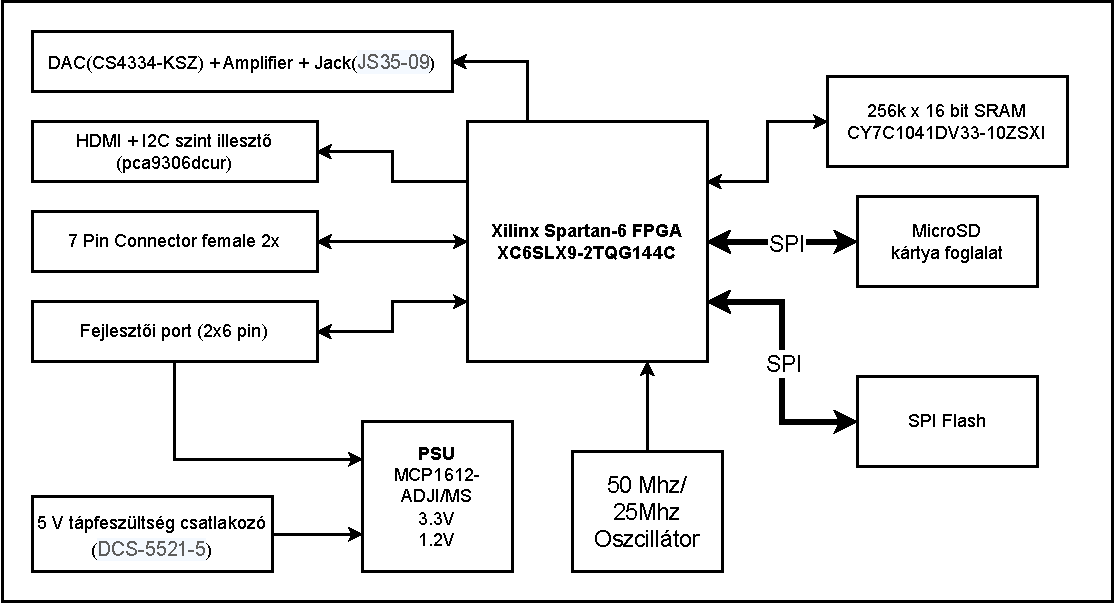
\includegraphics[width=150mm, keepaspectratio]{figures/NES-board-blockdiagram}
		\caption{NES kártya blokkdiagramja}
		\label{fig:PCB-blockdiagram}
	\end{figure}
	
	
	\subsection{Tápellátás}
	
	\subsection{Órajel források}
	
	\begin{table}[H]
		\footnotesize
		\centering
		\begin{tabular}{|l|l|}
			\hline
			\rowcolor[HTML]{C0C0C0} 
			\multicolumn{1}{|c|}{\cellcolor[HTML]{C0C0C0}{\color[HTML]{333333} \textbf{Órajel forrás}}} & \multicolumn{1}{c|}{\cellcolor[HTML]{C0C0C0}{\color[HTML]{333333} \textbf{FPGA láb}}} \\ \hline
			50 MHz-es oszcillátor                                                                       & P85                                                                                   \\ \hline
			Fejlesztői port CLK vonala                                                                  & P95                                                                                   \\ \hline
		\end{tabular}
		\caption{FPGA órajel forrásainak bekötése}
		\label{tab:FPGA-OSCpin}
	\end{table}
	
	\subsection{Memória - SRAM}
	
	\begin{table}[H]
		\footnotesize
		\centering
		\begin{tabular}{|lccccccccc|}
			\hline
			\rowcolor[HTML]{C0C0C0} 
			\multicolumn{10}{|l|}{\cellcolor[HTML]{C0C0C0}\textbf{Címbusz}}                                                                                                                                                                                                                                                                                                                                                                                                                                                                                                                                                                                                                                      \\ \hline
			\rowcolor[HTML]{EFEFEF} 
			\multicolumn{1}{|l|}{\cellcolor[HTML]{EFEFEF}SRAM}                            & \multicolumn{1}{c|}{\cellcolor[HTML]{EFEFEF}A0}                         & \multicolumn{1}{c|}{\cellcolor[HTML]{EFEFEF}A1}                         & \multicolumn{1}{c|}{\cellcolor[HTML]{EFEFEF}A2}                         & \multicolumn{1}{c|}{\cellcolor[HTML]{EFEFEF}A3}                         & \multicolumn{1}{c|}{\cellcolor[HTML]{EFEFEF}A4}                         & \multicolumn{1}{c|}{\cellcolor[HTML]{EFEFEF}A5}                         & \multicolumn{1}{c|}{\cellcolor[HTML]{EFEFEF}A6}                         & \multicolumn{1}{c|}{\cellcolor[HTML]{EFEFEF}A7}                         & A8   \\ \hline
			\rowcolor[HTML]{EFEFEF} 
			\multicolumn{1}{|l|}{\cellcolor[HTML]{EFEFEF}{\color[HTML]{333333} FPGA láb}} & \multicolumn{1}{c|}{\cellcolor[HTML]{EFEFEF}{\color[HTML]{333333} P47}} & \multicolumn{1}{c|}{\cellcolor[HTML]{EFEFEF}{\color[HTML]{333333} P46}} & \multicolumn{1}{c|}{\cellcolor[HTML]{EFEFEF}{\color[HTML]{333333} P45}} & \multicolumn{1}{c|}{\cellcolor[HTML]{EFEFEF}{\color[HTML]{333333} P44}} & \multicolumn{1}{c|}{\cellcolor[HTML]{EFEFEF}{\color[HTML]{333333} P43}} & \multicolumn{1}{c|}{\cellcolor[HTML]{EFEFEF}{\color[HTML]{333333} P34}} & \multicolumn{1}{c|}{\cellcolor[HTML]{EFEFEF}{\color[HTML]{333333} P33}} & \multicolumn{1}{c|}{\cellcolor[HTML]{EFEFEF}{\color[HTML]{333333} P32}} & P30  \\ \hline
			\multicolumn{1}{|l|}{SRAM}                                                    & \multicolumn{1}{c|}{A9}                                                 & \multicolumn{1}{c|}{A10}                                                & \multicolumn{1}{c|}{A11}                                                & \multicolumn{1}{c|}{A12}                                                & \multicolumn{1}{c|}{A13}                                                & \multicolumn{1}{c|}{A14}                                                & \multicolumn{1}{c|}{A15}                                                & \multicolumn{1}{c|}{A16}                                                & A17  \\ \hline
			\multicolumn{1}{|l|}{FPGA láb}                                                & \multicolumn{1}{c|}{P29}                                                & \multicolumn{1}{c|}{P7}                                                 & \multicolumn{1}{c|}{P6}                                                 & \multicolumn{1}{c|}{P5}                                                 & \multicolumn{1}{c|}{P2}                                                 & \multicolumn{1}{c|}{P1}                                                 & \multicolumn{1}{c|}{P139}                                               & \multicolumn{1}{c|}{P138}                                               & P137 \\ \hline
		\end{tabular}
		\caption{SRAM memória címbusz bekötése}
		\label{tab:FPGA-MEM-SRAMpin}
	\end{table}
		
	\begin{table}[H]
		\footnotesize
		\centering
		\begin{tabular}{|lcccccccc|}
			\hline
			\rowcolor[HTML]{C0C0C0} 
			\multicolumn{9}{|l|}{\cellcolor[HTML]{C0C0C0}\textbf{Adatbusz}}                                                                                                                                                                                                                                                                                                                                                                                                                                                                                                                                                                                  \\ \hline
			\rowcolor[HTML]{EFEFEF} 
			\multicolumn{1}{|l|}{\cellcolor[HTML]{EFEFEF}SRAM}                            & \multicolumn{1}{c|}{\cellcolor[HTML]{EFEFEF}D0}                         & \multicolumn{1}{c|}{\cellcolor[HTML]{EFEFEF}D1}                         & \multicolumn{1}{c|}{\cellcolor[HTML]{EFEFEF}D2}                         & \multicolumn{1}{c|}{\cellcolor[HTML]{EFEFEF}D3}                         & \multicolumn{1}{c|}{\cellcolor[HTML]{EFEFEF}D4}                         & \multicolumn{1}{c|}{\cellcolor[HTML]{EFEFEF}D5}                         & \multicolumn{1}{c|}{\cellcolor[HTML]{EFEFEF}D6}                         & D7                         \\ \hline
			\rowcolor[HTML]{EFEFEF} 
			\multicolumn{1}{|l|}{\cellcolor[HTML]{EFEFEF}{\color[HTML]{333333} FPGA láb}} & \multicolumn{1}{c|}{\cellcolor[HTML]{EFEFEF}{\color[HTML]{333333} P40}} & \multicolumn{1}{c|}{\cellcolor[HTML]{EFEFEF}{\color[HTML]{333333} P17}} & \multicolumn{1}{c|}{\cellcolor[HTML]{EFEFEF}{\color[HTML]{333333} P21}} & \multicolumn{1}{c|}{\cellcolor[HTML]{EFEFEF}{\color[HTML]{333333} P22}} & \multicolumn{1}{c|}{\cellcolor[HTML]{EFEFEF}{\color[HTML]{333333} P23}} & \multicolumn{1}{c|}{\cellcolor[HTML]{EFEFEF}{\color[HTML]{333333} P24}} & \multicolumn{1}{c|}{\cellcolor[HTML]{EFEFEF}{\color[HTML]{333333} P26}} & {\color[HTML]{333333} P27} \\ \hline
			\multicolumn{1}{|l|}{SRAM}                                                    & \multicolumn{1}{c|}{D8}                                                 & \multicolumn{1}{c|}{D9}                                                 & \multicolumn{1}{c|}{D10}                                                & \multicolumn{1}{c|}{D11}                                                & \multicolumn{1}{c|}{D12}                                                & \multicolumn{1}{c|}{D13}                                                & \multicolumn{1}{c|}{D14}                                                & D15                        \\ \hline
			\multicolumn{1}{|l|}{FPGA láb}                                                & \multicolumn{1}{c|}{P8}                                                 & \multicolumn{1}{c|}{P9}                                                 & \multicolumn{1}{c|}{P10}                                                & \multicolumn{1}{c|}{P11}                                                & \multicolumn{1}{c|}{P12}                                                & \multicolumn{1}{c|}{P14}                                                & \multicolumn{1}{c|}{P15}                                                & P16                        \\ \hline
		\end{tabular}
		\caption{SRAM memória adatbusz bekötése}
		\label{tab:FPGA-DATA-SRAMpin}
	\end{table}

	\begin{table}[H]
		\footnotesize
		\centering
		\begin{tabular}{|llllcc|}
			\hline
			\multicolumn{6}{|l|}{\cellcolor[HTML]{C0C0C0}\textbf{Vezérlő jelek}}                                                                                \\ \hline
			\multicolumn{1}{|l|}{SRAM}     & \multicolumn{1}{l|}{CSn} & \multicolumn{1}{l|}{WEn} & \multicolumn{1}{l|}{OEn}  & \multicolumn{1}{c|}{LBn}  & UBn  \\ \hline
			\multicolumn{1}{|l|}{FPGA láb} & \multicolumn{1}{l|}{P41} & \multicolumn{1}{l|}{P35} & \multicolumn{1}{l|}{P140} & \multicolumn{1}{c|}{P142} & P141 \\ \hline
		\end{tabular}
		\caption{SRAM memória vezérlő jelek bekötése}
		\label{tab:FPGA-CONTROL-SRAMpin}
	\end{table}

	
	\subsection{Soros Flash memória}
	
	\subsection{Digital Analog Converter és erősítő}
	
	\subsection{HDMI és I2C szint illesztő}
	
	\begin{figure}[H]
	\begin{minipage}[]{\textwidth}
		\begin{minipage}[b]{0.39\textwidth}
			\centering
			\includegraphics[width=55mm, keepaspectratio]{figures/hdmi-Pinout}
			\captionof{figure}{aljzat anya}
			\label{fig:HDMI-pinout}
		\end{minipage}
		\hfill
		\begin{minipage}[b]{0.59\textwidth}
			\footnotesize
			\centering
			\begin{tabular}{|l|c|l|c|}
				\hline
				\rowcolor[HTML]{C0C0C0} 
				\textbf{Funkció}  & \multicolumn{1}{l|}{\cellcolor[HTML]{C0C0C0}{\color[HTML]{333333} \textbf{Láb}}} & \textbf{Funkció}  & \multicolumn{1}{l|}{\cellcolor[HTML]{C0C0C0}{\color[HTML]{333333} \textbf{Láb}}} \\ \hline
				TMDS Data2+       & 1                                                                                & TMDS Clock Shield & 11                                                                               \\ \hline
				TMDS Data2 Shield & 2                                                                                & TMDS Clock-       & 12                                                                               \\ \hline
				TMDS Data-        & 3                                                                                & CEC               & 13                                                                               \\ \hline
				TMDS Data1+       & 4                                                                                & Reserved          & 14                                                                               \\ \hline
				TMDS Data1 Shield & 5                                                                                & SCL               & 15                                                                               \\ \hline
				TMDS Data1-       & 6                                                                                & SDA               & 16                                                                               \\ \hline
				TMDS Data0+       & 7                                                                                & DDC/CEC Ground    & 17                                                                               \\ \hline
				TMDS Data0 Shield & 8                                                                                & +5 V Power        & 18                                                                               \\ \hline
				TMDS Data0-       & 9                                                                                & Hot Plug Detected & 19                                                                               \\ \hline
				TMDS Clock+       & 10                                                                               &                   & \multicolumn{1}{l|}{}                                                            \\ \hline
			\end{tabular}
			\captionof{table}{HDMI pin kiosztás}
			\label{tab:HDMI-pinout}
		\end{minipage}
	\end{minipage}
	\end{figure} 
	
	\subsection{Eredeti kontroller portok}
	
	\subsection{MicroSD kártya}
	
	\subsection{FPGA konfigurációs módok}
	
	\begin{table}[H]
		\footnotesize
		\centering
		\begin{tabular}{|c|c|l|}
			\hline
			\rowcolor[HTML]{C0C0C0} 
			\textbf{\begin{tabular}[c]{@{}c@{}}Jumper\\ állása\end{tabular}} & {\color[HTML]{333333} \textbf{\begin{tabular}[c]{@{}c@{}}Konfigurációs \\ mód\end{tabular}}} & \multicolumn{1}{c|}{\cellcolor[HTML]{C0C0C0}\textbf{Leírás}}                                                                                                                          \\ \hline
			\rowcolor[HTML]{FFFFFF} 
			\raisebox{-.5\height}{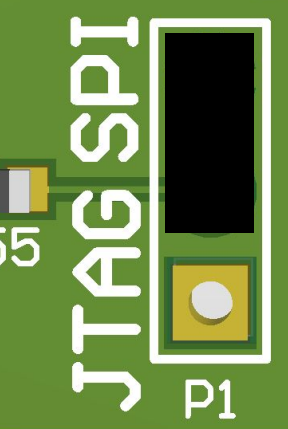
\includegraphics[width=10mm, keepaspectratio]{figures/SPI-jumper}}                                                                & JTAG                                                                                         & Az FPGA-t a JTAG interfacen keresztül kell felkonfigurálni.                                                                                                                           \\ \hline
			\rowcolor[HTML]{FFFFFF} 
			\raisebox{-.5\height}{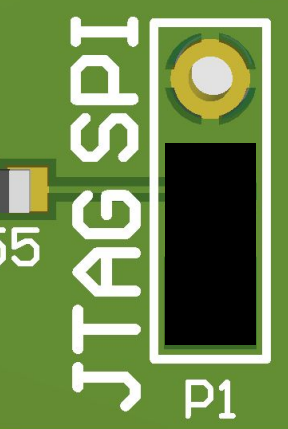
\includegraphics[width=10mm, keepaspectratio]{figures/JTAG-jumper}}                                                                & SPI                                                                                          & \begin{tabular}[c]{@{}l@{}}Az FPGA az SPI buszos soros FLASH memóriából konfigurálja \\ fel magát a tápfeszültség bekapcsolása vagy a PROG gomb \\ megnyomását követően.\end{tabular} \\ \hline
		\end{tabular}
		\caption{Fejlesztői port bekötése}
		\label{tab:FPGA-config}
	\end{table}
	%TODO fix jumper heights if you have time
	\subsection{LOGSYS fejlesztői port}
	
	\begin{figure}[H]
		\begin{minipage}[]{\textwidth}
			\begin{minipage}[b]{0.49\textwidth}
				\centering
				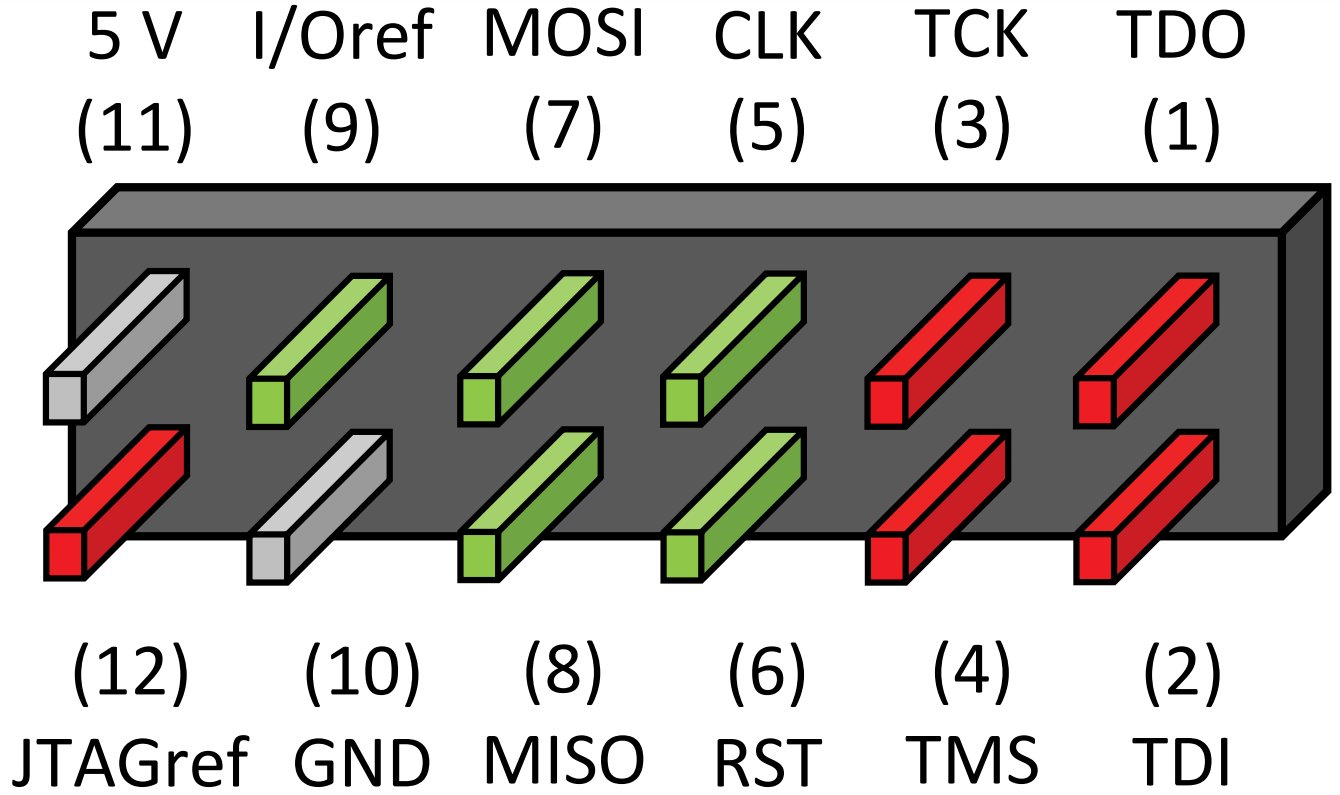
\includegraphics[width=50mm, keepaspectratio]{figures/DEV-port}
				\captionof{figure}{Fejlesztői port tűsorának kiosztása}
				\label{fig:DEV-port}
			\end{minipage}
			\hfill
			\begin{minipage}[b]{0.49\textwidth}
				\footnotesize
				\centering
				\begin{tabular}{|l|l|l}
					\cline{1-2}
					\rowcolor[HTML]{C0C0C0} 
					\multicolumn{1}{|c|}{\cellcolor[HTML]{C0C0C0}\textbf{jel}} & \multicolumn{1}{c|}{\cellcolor[HTML]{C0C0C0}{\color[HTML]{333333} \textbf{Irány}}} & \multicolumn{1}{c}{\cellcolor[HTML]{C0C0C0}\textbf{FPGA láb}} \\ \hline
					\rowcolor[HTML]{FFFFFF} 
					MOSI                                                       & bemenet                                                                            & \multicolumn{1}{l|}{\cellcolor[HTML]{FFFFFF}P104}             \\ \hline
					\rowcolor[HTML]{FFFFFF} 
					MISO                                                       & kimenet                                                                            & \multicolumn{1}{l|}{\cellcolor[HTML]{FFFFFF}P144}             \\ \hline
					CLK                                                        & bemenet                                                                            & \multicolumn{1}{l|}{P95}                                      \\ \hline
					RST                                                        & bemenet                                                                            & \multicolumn{1}{l|}{P94}                                      \\ \hline
				\end{tabular}
				\captionof{table}{Fejlesztői port bekötése}
				\label{tab:DEV-pinout}
			\end{minipage}
		\end{minipage}
	\end{figure} 
	

\section{PCB layout}
	\subsection{Komponensek elhelyezése}
	%TODO komponensek game consolos kialalakítás végett hordozhatóság
	\begin{figure}[H]
		\centering
		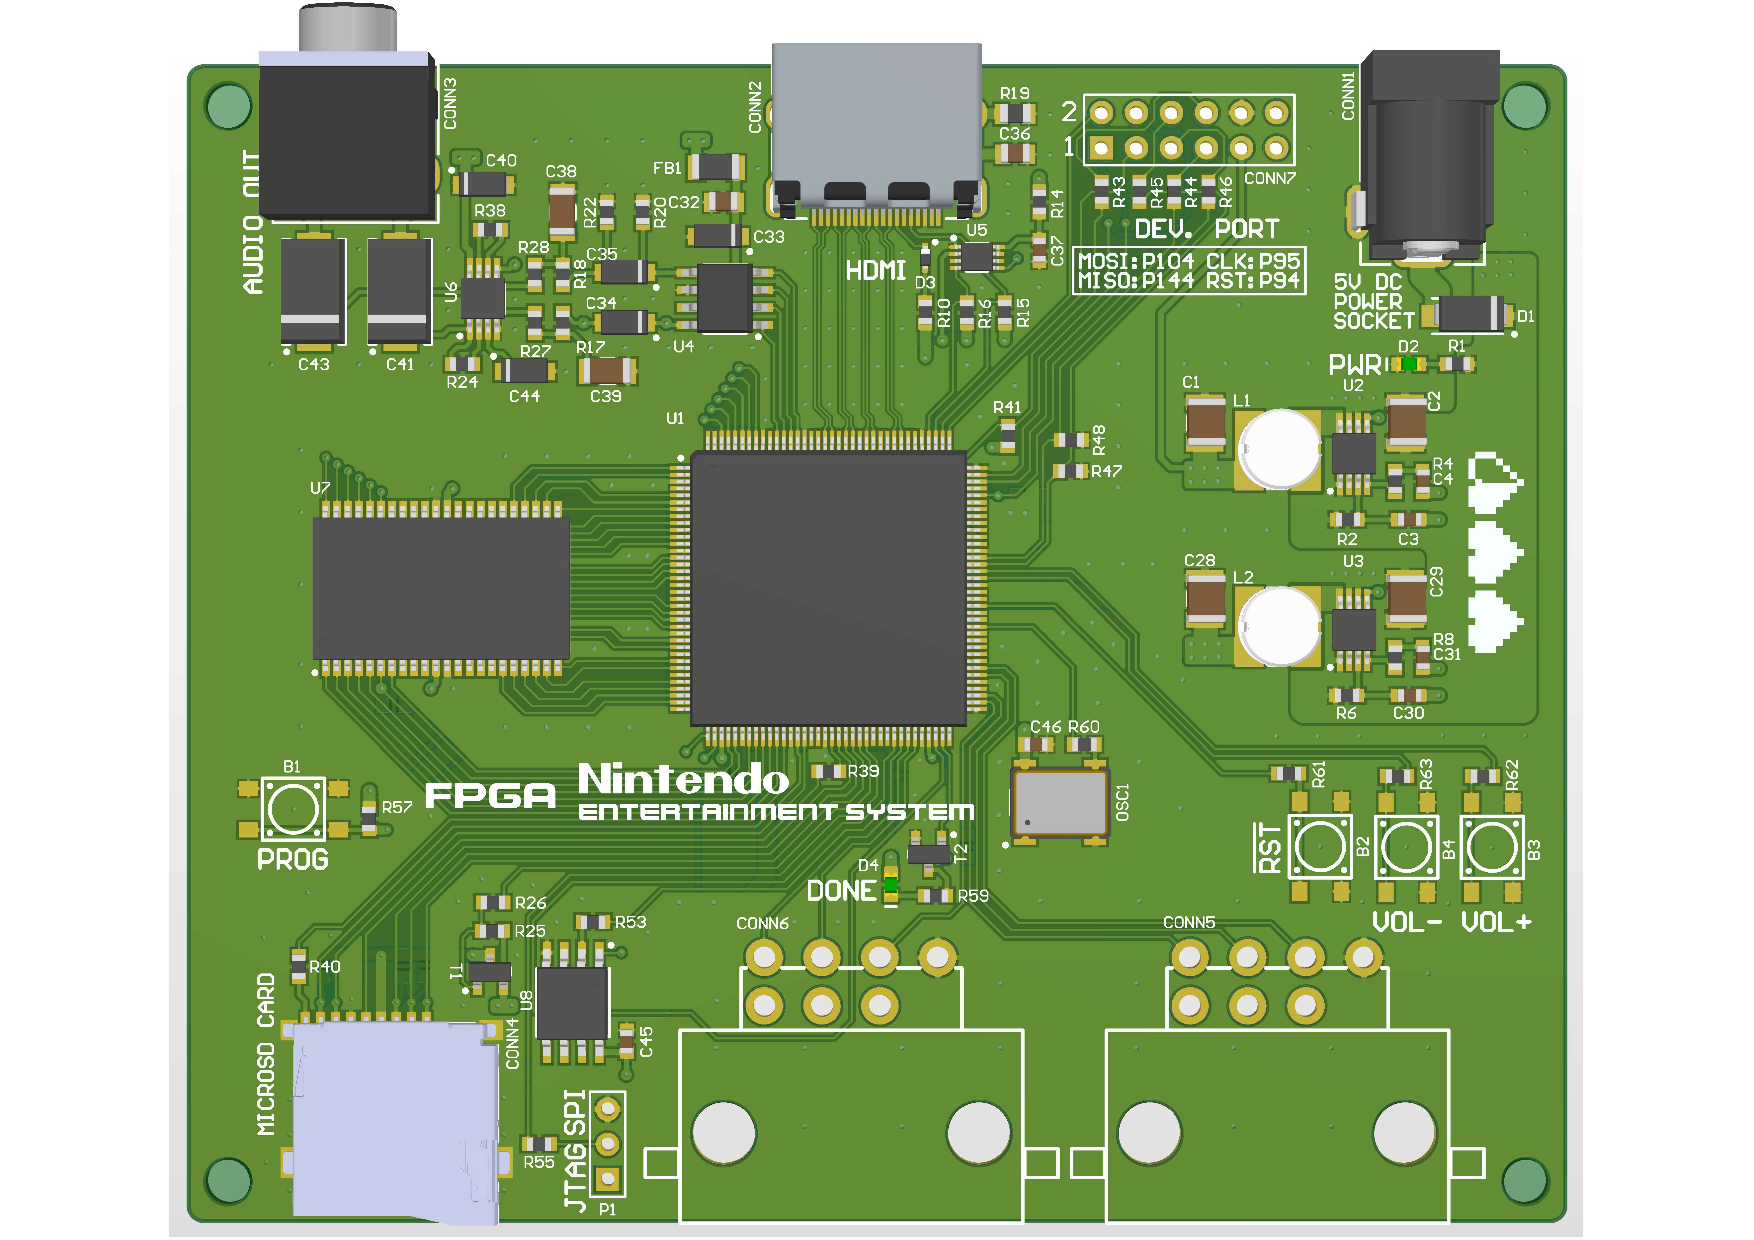
\includegraphics[width=100mm, keepaspectratio, angle=90]{figures/Top}
		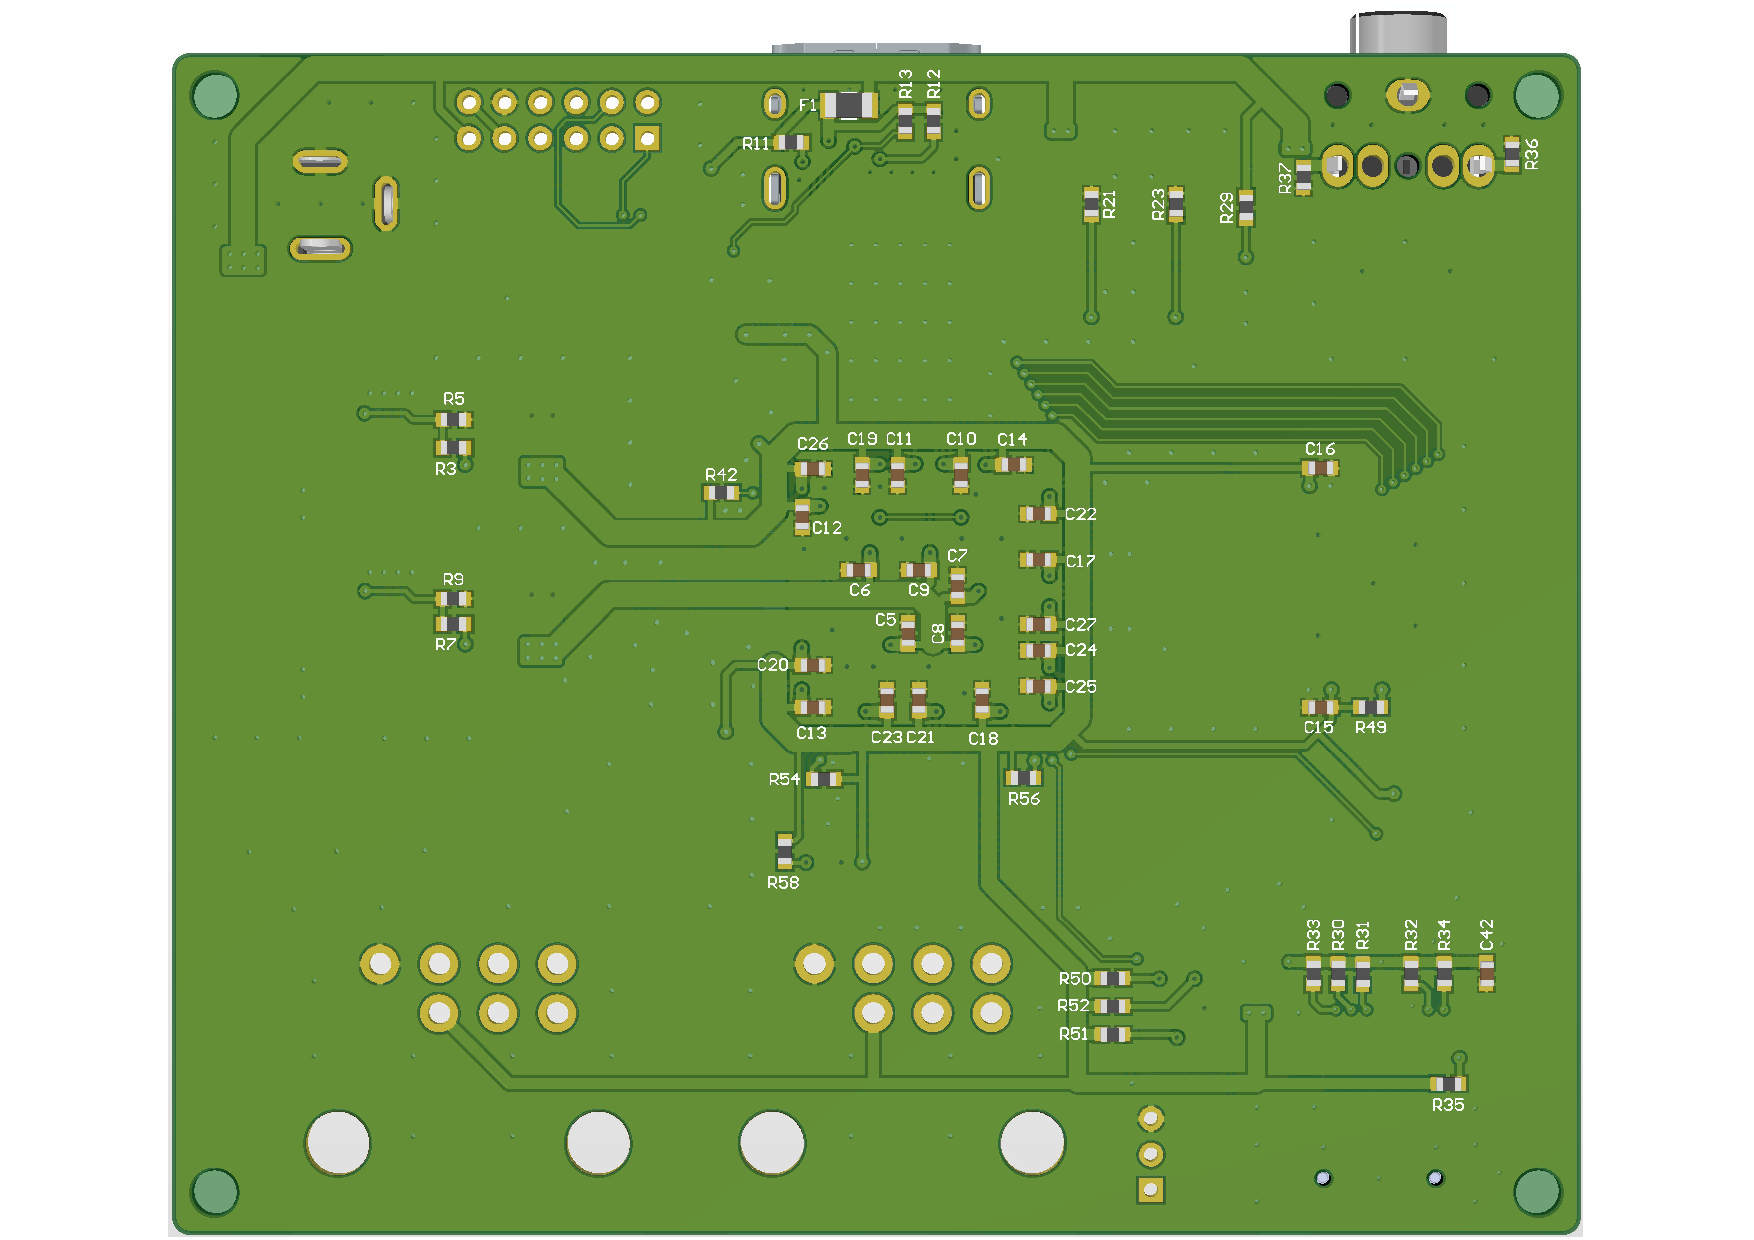
\includegraphics[width=100mm, keepaspectratio, angle=90]{figures/Bottom}\\\vspace{5mm}
		\caption{3D PCB rajzolat} 
		\label{fig:PCB-3D}
	\end{figure}
	\subsection{Réteg beállítások}
	
	\subsection{Coplanar differential pair rooting}
	
	\subsection{Táp vonalak kialakítása}
	
	
	
	

